\lysh{33711}{4}

\begin{alist}
\item Το τριώνυμο $x^2 - 2x - 8$ έχει $\alpha = 1, \beta = -2, \gamma = -8$ και διακρίνουσα
\[\Delta = \beta^2 - 4\alpha\gamma = (-2)^2 - 4 \cdot 1 \cdot (-8) = 4 + 32 = 36 > 0.\]
Οι ρίζες του τριωνύμου είναι οι:
\[x_{1,2} = \dfrac{-\beta \pm \sqrt{\Delta}}{2\alpha} = \dfrac{-(-2) \pm \sqrt{36}}{2 \cdot 1} = \dfrac{2 \pm 6}{2} = \begin{cases} 4 \\ -2 \end{cases}.\]

Το πρόσημο του τριωνύμου φαίνεται στον παρακάτω πίνακα:

\begin{center}
\begin{tikzpicture}
\tikzset{t style/.style = {style = dashed}}
\tkzTabInit[color,lgt=3,espcl=2,colorC = maincolor!40,
colorL = maincolor!20,
colorV = maincolor!40]%
{$x$ / .8,$x^2 - 2x - 8$ /0.8}%
{$-\infty$,$-1$,$2$,$+\infty$}%
\tkzTabLine{ , $+$, z
, $-$ , z
, $+$ , }
\end{tikzpicture}
\end{center}

Από τον πίνακα προσήμων συμπεραίνουμε ότι:
\[x^2 - 2x - 8 < 0 \Leftrightarrow -2 < x < 4 \Leftrightarrow x \in (-2, 4)\]
και
\[x^2 - 2x - 8 > 0 \Leftrightarrow (x < -2 \text{ ή } x > 4) \Leftrightarrow x \in (-\infty, -2) \cup (4, +\infty).\]

\item Για να βρούμε το πρόσημο της παράστασης $\kappa^2 - 2\kappa - 8$ πρέπει να γνωρίζουμε σε ποιο
από τα διαστήματα του ερωτήματος $\alpha)$ ανήκει ο $\kappa = -\dfrac{8889}{4444}$. Συγκρίνουμε τον $\kappa$ με το $-2$:
\[\kappa - (-2) = -\dfrac{8889}{4444} + 2 = -\dfrac{8889}{4444} + \dfrac{8888}{4444} = -\dfrac{1}{4444} < 0.\]
Άρα, $\kappa - (-2) < 0 \Leftrightarrow \kappa < -2$. Οπότε, από τον πίνακα του ερωτήματος $\alpha)$ συμπεραίνουμε
ότι $\kappa^2 - 2\kappa - 8 > 0$.

\item Η δοθείσα παράσταση γράφεται:
\[\mu^2 - 2|\mu| - 8 = |\mu|^2 - 2|\mu| - 8.\]
Επομένως προκύπτει από το αρχικό τριώνυμο για $x = |\mu|$.
Επίσης έχουμε ότι:
\[-4 < \mu < 4 \Leftrightarrow |\mu| < 4 \Leftrightarrow 0 \le |\mu| < 4.\]
Από τον πίνακα προσήμων του ερωτήματος $\alpha)$ διαπιστώνουμε ότι για $0 \le |\mu| < 4$ είναι:
$|\mu|^2 - 2|\mu| - 8 < 0$.
\end{alist}
